\chapter{Extracting the data you want from a text file}
\label{assignment:extracting} 

\begin{flushright}
	\parbox{8cm}
		{
		\begin{flushright}
		\rule{8cm}{0.5pt}\\
		\vspace*{5mm}
		\sffamily \
		Reading:\\
		\href{http://matplotlib.sourceforge.net/}{Matplotlib Web Site}
		
		\vspace*{5mm}
		\rule{8cm}{0.5pt}
		\end{flushright}
		}
\end{flushright}


\section{Statement of the problem}\label{sec:statement01}
Here's a problem that you frequently encounter as a scientist: you use a data acquisition system to measure some phenomenon, and although the data that gets written to disk is merely alphanumeric text (technical term is ascii---American Standard Code for Information Interchange for those of you who are interested), the format of this ascii file is not of the form that scientific graphics tools can easily plot.

What do you do? 

One option is to import it into a spreadsheet, and use the functionality of a spreadsheet to extract the data points you want. I won't do this, because I don't know enough about spreadsheet functionality---I suspect most physicists are in the same boat on this. 

Another option is to manually read the data file and type it by hand. This is fine for a small data file, but introduces the inevitable typo(s), and is a totally absurd approach to a data file with millions of data points. 

What we need is a way to read in a data file, extract what we need and write out a new data file in a more convenient format; and this method should work equally well for a small file or a data set with millions of points.

\section{An example}\label{sec:example}

Let's make this more concrete with an example. Table~\ref{tab:data} shows a short section of a 1000 line data file. The data is from an optical switch used to measure the period of a pendulum. 

\begin{table}
\caption{A short sample from the data set.}\label{tab:data}
\vspace*{3mm}
\begin{tabular}{ccc}
\toprule
time (s)			& state	& period (s)\\
\midrule
0.5389116	& \hspace*{5mm}1	\hspace*{5mm} & ---\\
0.6551832	&	\hspace*{5mm}0	\hspace*{5mm} &\\
2.2663992	&	\hspace*{5mm}1	\hspace*{5mm} &\\
2.3827892	&	\hspace*{5mm}0	 \hspace*{5mm}&\\
4.0025032	&	\hspace*{5mm}1	 \hspace*{5mm}&	3.4635916\\
4.118984	&	\hspace*{5mm}0	\hspace*{5mm} & \\
5.7299832	&\hspace*{5mm}1	\hspace*{5mm} &	 \\
5.8465832	&\hspace*{5mm}0 \hspace*{5mm} &	 \\
7.4661176	&\hspace*{5mm}1	 \hspace*{5mm}& 3.4636144\\
7.5827832	&\hspace*{5mm}0	\hspace*{5mm} & \\
\bottomrule
\vspace*{4mm}
\end{tabular}
\end{table}
A laser beam is sent through the air to photodiode, and a digital signal is recorded each time the pendulum enters or leaves a laser beam. Figure~\ref{fig:opticalSwitch} schematically shows the pendulum breaking the laser beam at time $t_a$, leaving the beam at $t_b$, breaking it at $t_c$, and leaving the beam at $t_d$. The next breaking of the beam at time $t_e$ (not shown) will then allow one to calculate the period as $T = t_e - t_a$. 

The problem here is that the format of this data file is not readily readable by many plotting programs. What we'd like to do is filter through this data only extracting the data where we have a period measurement. When you do so, you'll then have a two column data set with time and period values only. Then, it is a simple matter to read the data file and plot it with (for example) a tool like {\em gnuplot} or (as in Figure~\ref{fig:Output}), {\em Matplotlib}. 
\begin{figure}[ht]
\sidecaption
  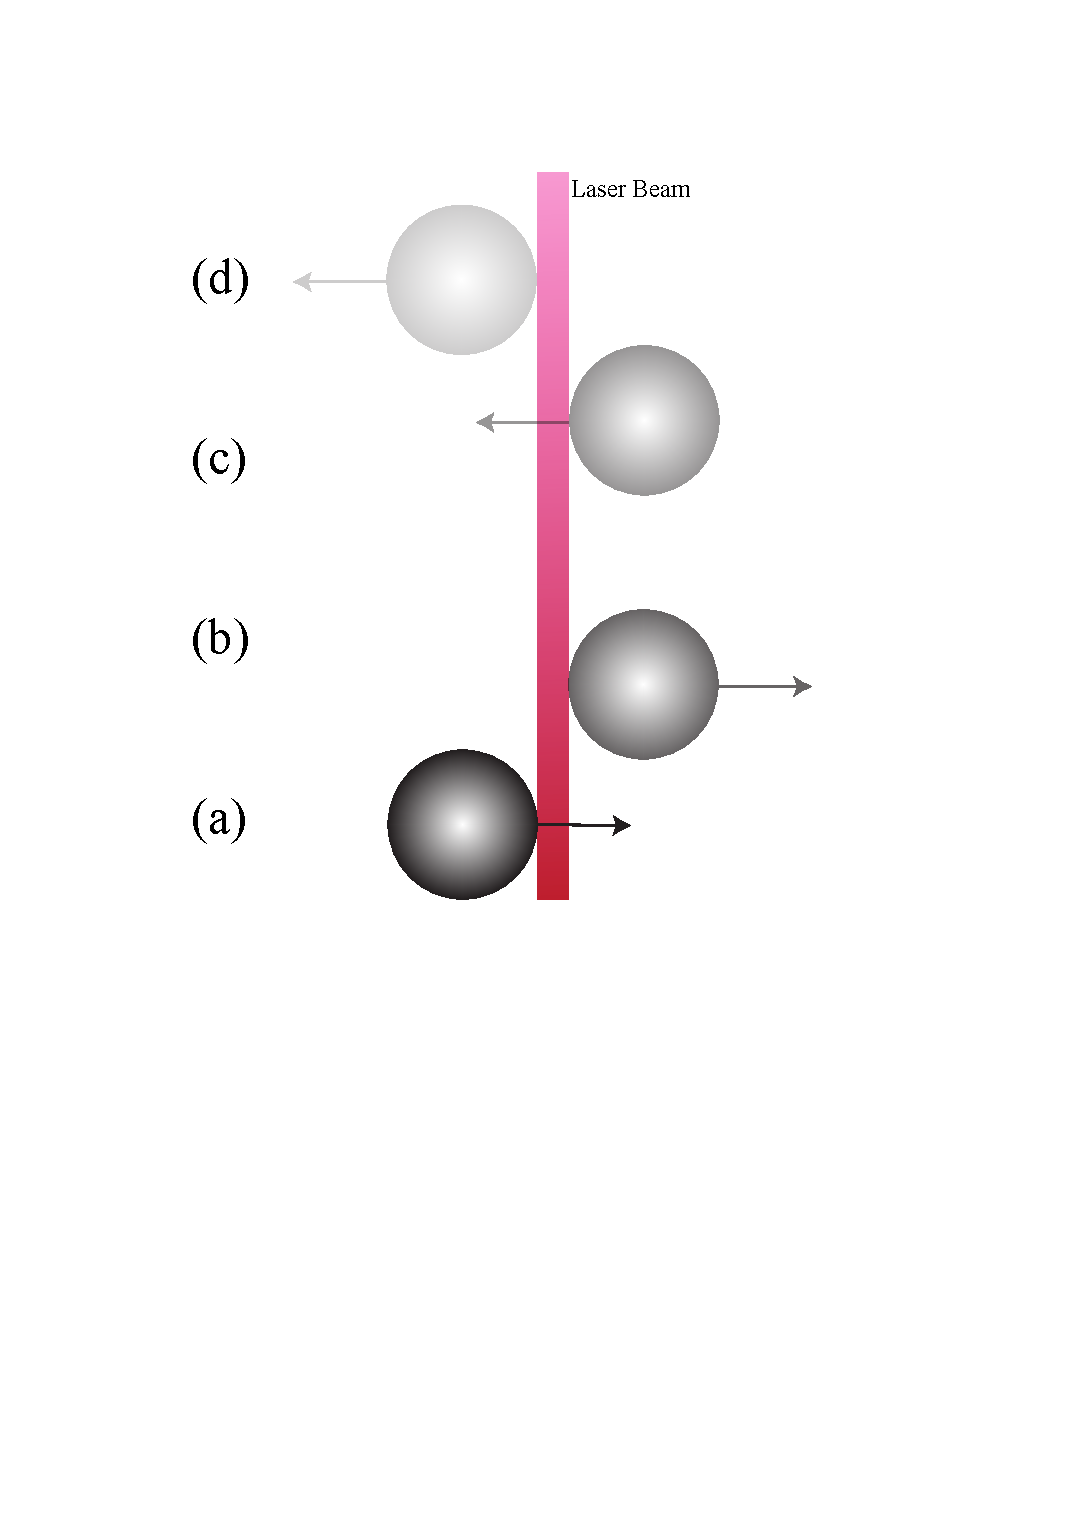
\includegraphics[width=.3\linewidth]{Figures/extractingData/OpticalSwitch.png}%
  \caption{The idea behind an optical switch---each time the pendulum enters or leaves the beam, a digital timing signal is recorded. In the figure, the pendulum is drawn a four different times; on the 5th crossing (not shown), one will have enough information to calculate the period.}
  \label{fig:opticalSwitch}%
\end{figure}

\begin{figure}[htb]
 \includegraphics[width=0.85\linewidth]{Figures/extractingData/Output.png}%
  \caption{A plot (using Matplotlib) of the period vs time data from the full data set. Notice that Matplotlib automatically pulled out 3.462 s from the period axis on the left, so that the vertical tics are space 0.4 ms apart, and over the course of 850 seconds, the period of the pendulum only changed by about 1 mS.}
  \label{fig:Output}%
\end{figure}


\section{Details for this Assignment }\label{sec:task1}
\begin{enumerate}
	\item Read the file {\textsf PeriodData.dat}, and extract only lines with actual period values. Create an output file called {\textsf Filtered.dat} (which will go in your data folder---see Appendix~\ref{app:submission} for submission guidelines). I've posted one way (not the most elegant, but it works) to do this at \href{http://people.usm.maine.edu/pauln/261downloads.html}{http://people.usm.maine.edu/pauln/261downloads.html} in file filter.py
	\item Plot this data from within your script using Matplotlib. I suggest you go to the Matplotlib gallery, find a simple x-y plot similar to what you want, and examine the code needed to create the plot.
	\item Once you create the plot on the screen, you can click the disk icon on the plot to save it to disk (in your \verb&LaTeX/Figures& folder) as a .png or a .pdf file. 
	\item As a part two to this exercise, still using the data from periodData.txt (at \href{http://people.usm.maine.edu/pauln/261downloads.html}{http://people.usm.maine.edu/pauln/261downloads.html}) create a data file with all possible periods extracted; i.e. you can calculate the period as the difference in time between every 4th crossing:
	$$ \mathrm{Period}_i = t_{i+4} - t_i$$
In this scheme, you'll end up with roughly three times as many period measurements. Create a new output file called \textsf{tripleFiltered.dat}, and plot this data file as you did with \textsf{filtered.dat}. Keep in mind that you will have to modify your program to produce this data file. 
	\item Now write a short \LaTeX\ report about what you did. This is \textbf{not}
	a formal report, but simply an exercise to get your Linux/Python/LaTeX feet wet. When you're done, you'll have had experience with the three main tools we'll work with all semester, so the rest of the term will polish and deepen your familiarity with these tools.
	\item Don't forget to submit your completed assignment according to the format specified in Appendix~\ref{app:submission}. Your python scripts for part 1 and part 2 should of course be in your code folder. You do not have to use the code I posted to do part 1---if you have a better way, please feel free to ignore my code, and I'll include a handout of all the different methods people used when I hand back your assignment submissions. 
\end{enumerate}

